\subsection{Der Spawner}
\todo{Noch in Arbeit}
\todo{Deadline: 26.06.}

\begin{figure}[!hb]
	\centering
	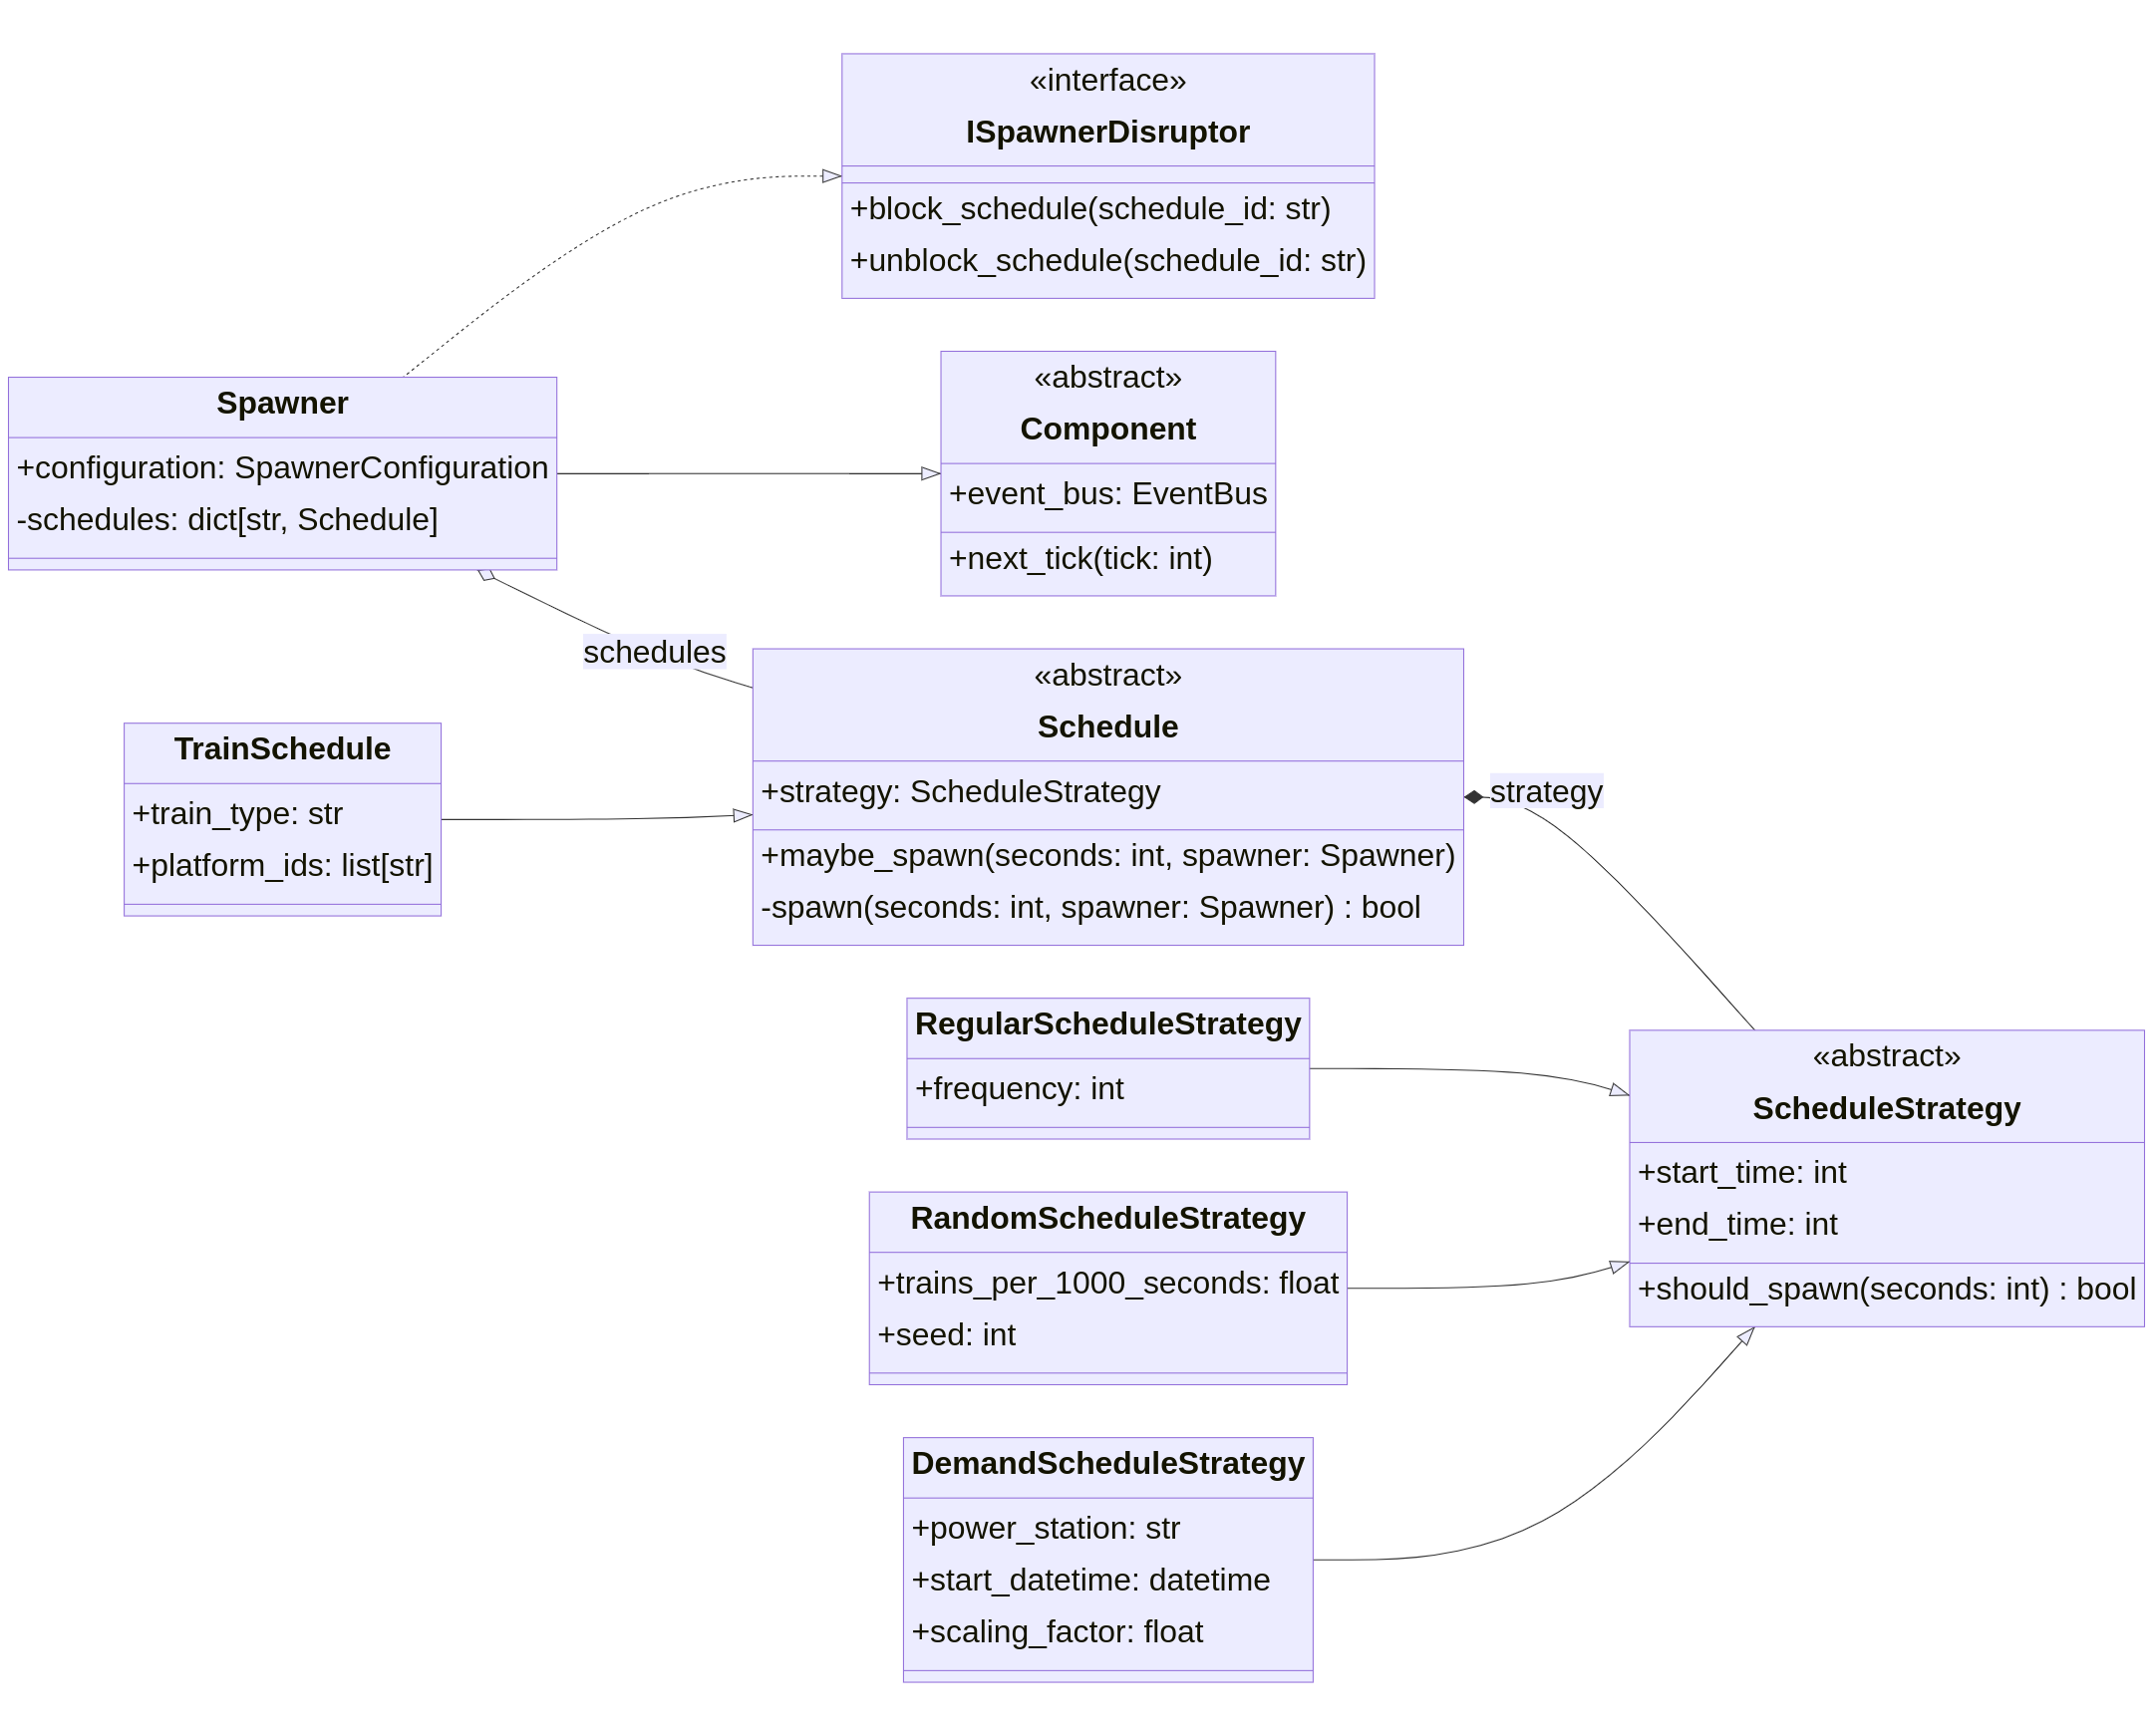
\includegraphics[width=0.75\linewidth]{images/diagrams/spawner-class.png}
	\caption{Klassendiagramm Spawner}
	\label{fig:spawner-class}
\end{figure}

\begin{figure}[!hb]
	\centering
	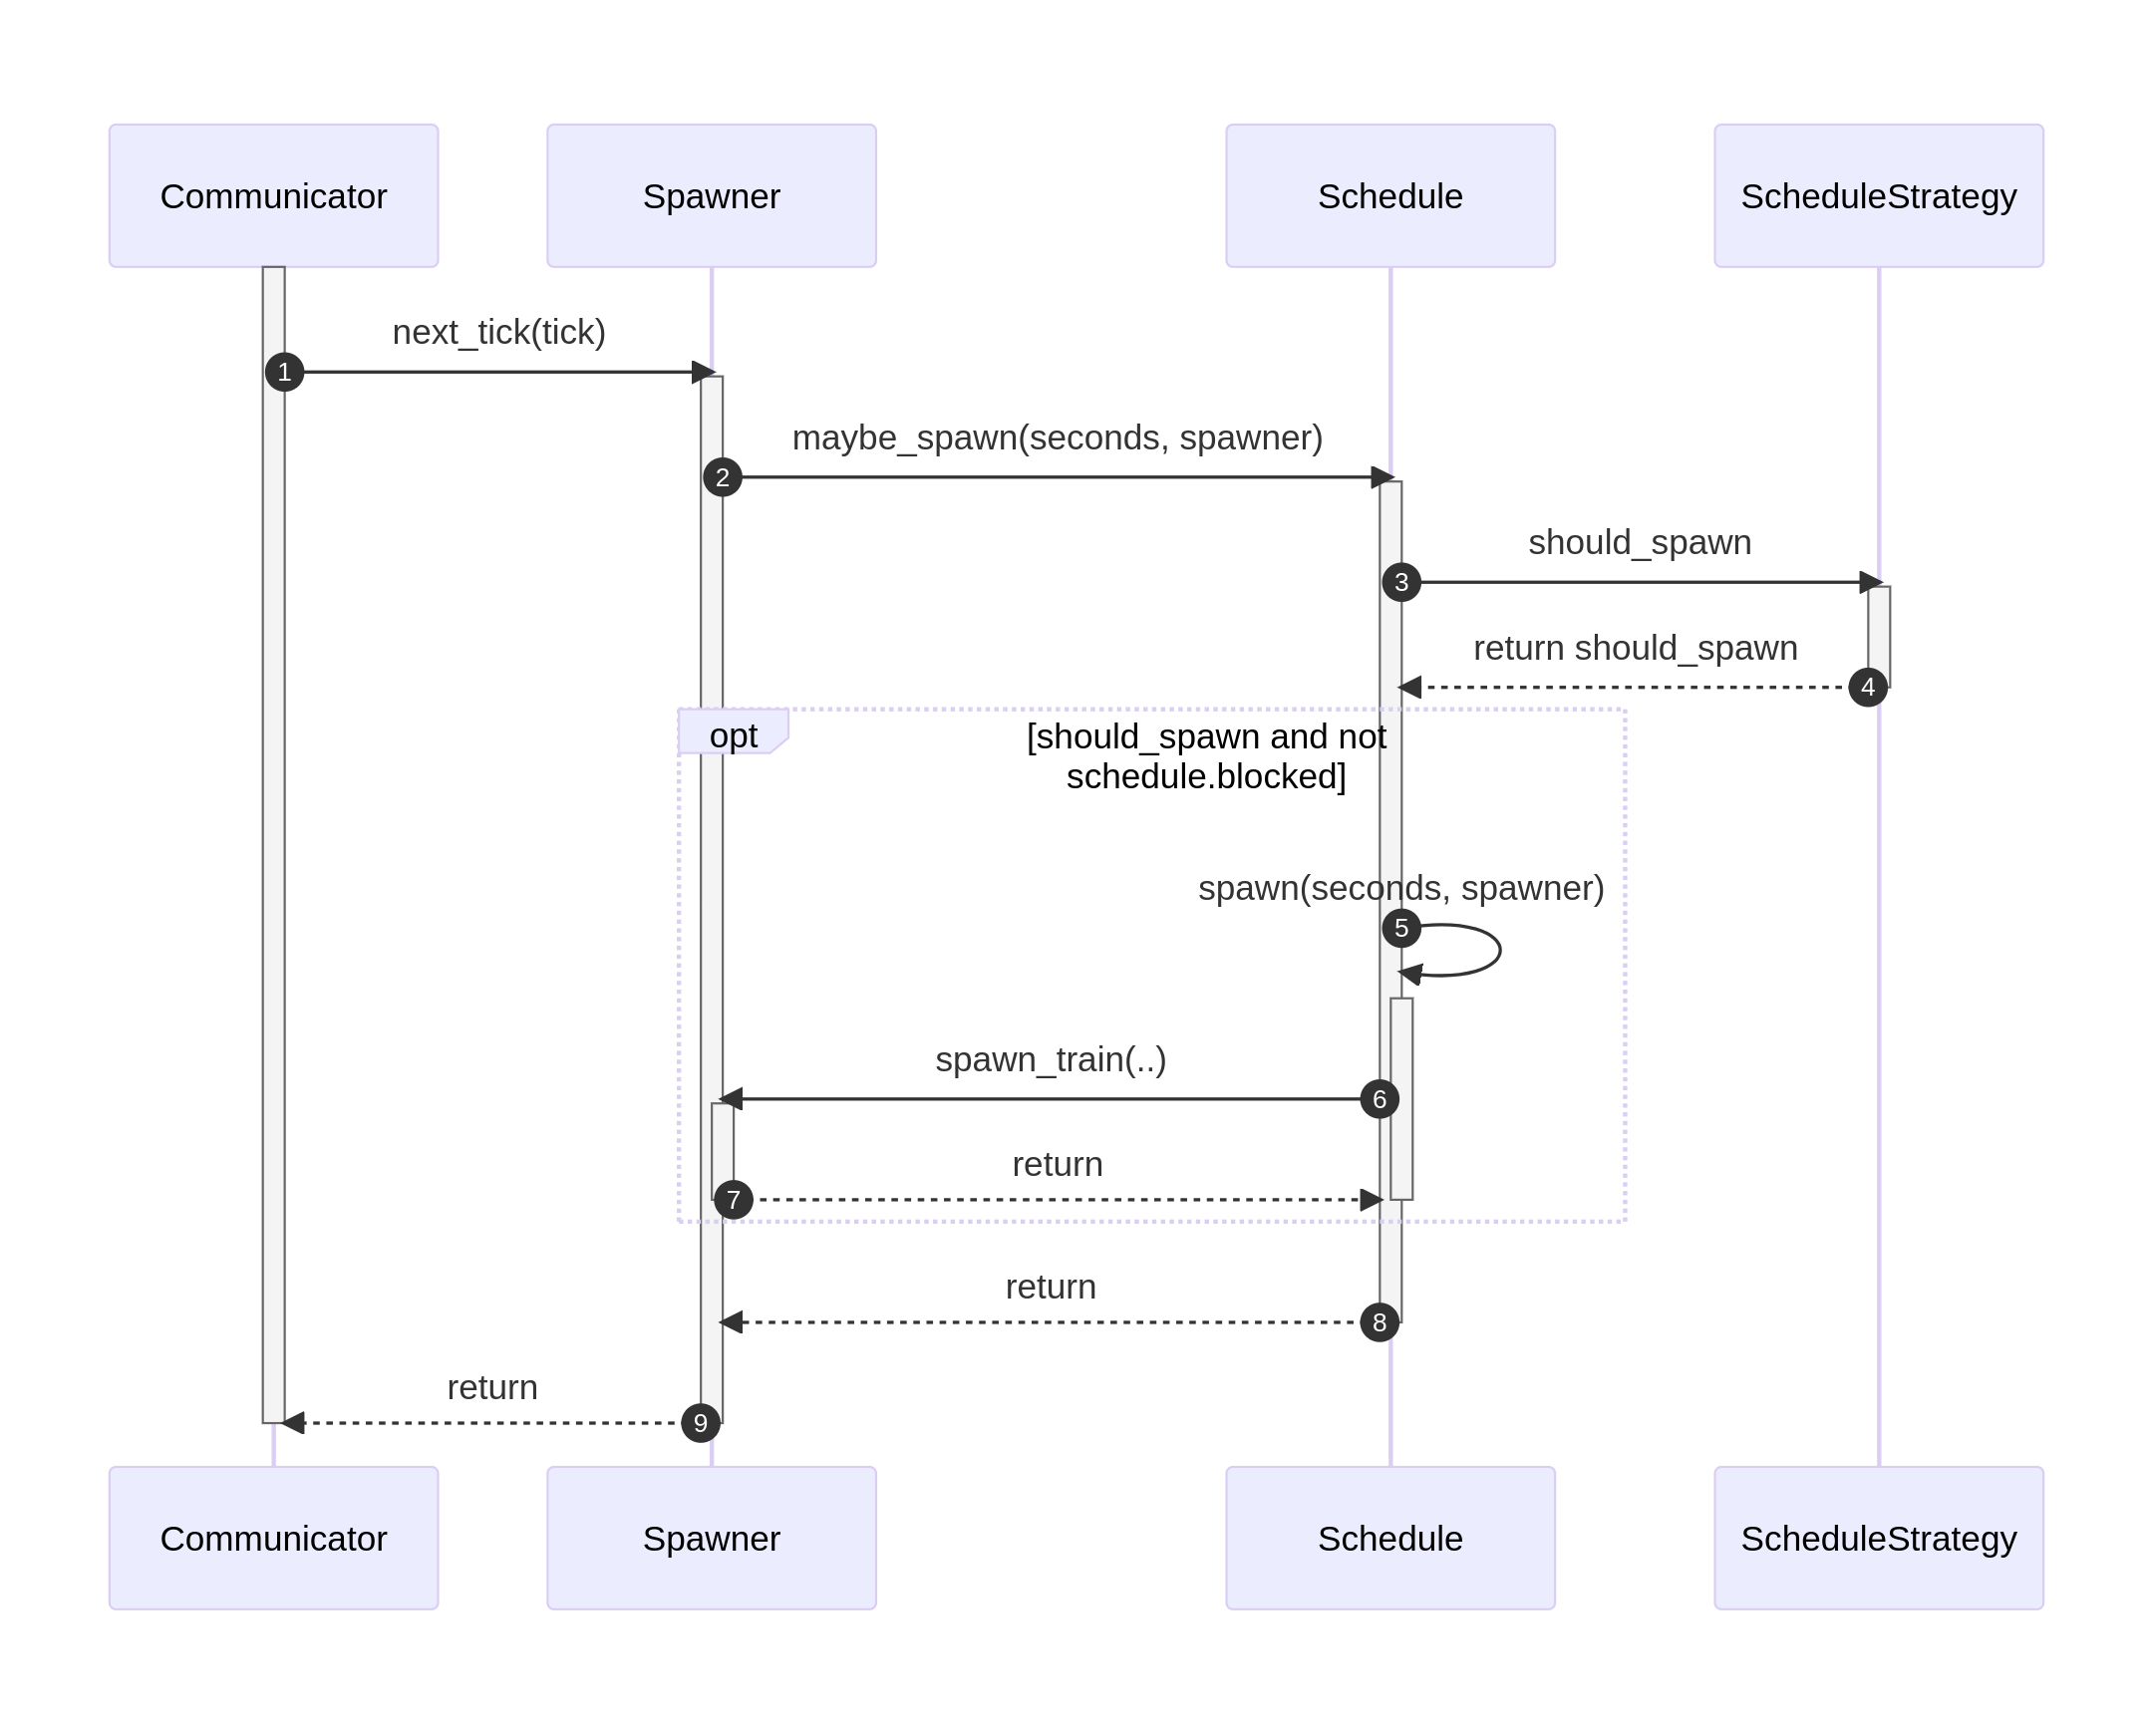
\includegraphics[width=0.75\linewidth]{images/diagrams/spawner-seq.png}
	\caption{Sequenzdiagramm Spawner}
	\label{fig:spawner-seq}
\end{figure}

Unser System simuliert die Interaktion von Zügen und diese Züge müssen zu bestimmten Zeiten instanziiert werden. Jedoch könne wir keine SUMO-Flows für das Spawning verwenden, weil diese nicht in der Lage sind, das von uns gewünschte Fahrstraßenverhalten abzubilden. Deshalb haben wir die Spawner-Komponente entwickelt, welche mit Hilfe einer Liste von Stationen, einen Zug in die Simulation setzt.

Der *Spawner* erbt wie die meisten anderen Teile der Software von *Component*, um über `next\_tick` auf die nächste Iteration der Simulation reagieren zu können. Außerdem erhält der Spawner somit Zugriff auf den *EventBus*, welcher es ermöglicht, Events zu emittieren und auf emittierte Events zu reagieren.

Der *Spawner* hält eine Liste von *Schedules*. Ein *Schedule* repräsentiert eine Menge von SUMO-Entitäten, den Weg, den diese in der Simulation zurücklegen sowie die Zeitpunkte, zu denen die Entitäten instanziiert werden. Weiterhin kann ein *Schedule* vom *FaultInjector* geblockt werden, um die Erzeugung von Entitäten für einen bestimmtes Zeitintervall zu unterbinden.

Für einen *Schedule* können Spezialisierungen angelegt werden, um auf die Besonderheiten verschiedener Arten von Entitäten Rücksicht zu nehmen. So müssen z.B. bei der Erzeugung von Fußgängern zum Teil andere Faktoren berücksichtigt werden, als bei der Erzeugung von Zügen. Daher haben wir uns entschieden, die Spezialisierung *TrainSpawner*, zur Erzeugung der Züge zu verwenden. Ein *PedestrianSpawner* war geplant, konnte jedoch im Rahmen des Projektes nicht mehr umgesetzt werden. Der *TrainSchedule* enthält zusätzlich Informationen über den Zugtyp (z.B. Personenzug oder Güterzug), die Route, die der Zug abfährt und dessen Haltepunkte. Diese Route ist als Liste von IDs hinterlegt, welche die anzufahrenden Bahnsteige referenzieren.

Im Rahmen unseres Projektes untersuchten wir drei verschiedene Möglichkeiten, die Erzeugungszeitpunkte für Entitäten festzulegen. Dies waren eine regelmäßige, eine zufällige und eine bedarfsorientierte Erzeugung. Ein naiver Ansatz, um diese Möglichkeiten in der Architektur widerzuspiegeln, ist es, Vererbung zu verwenden. Dieser Ansatz ist allerdings nicht skalierbar, da $n$ Möglichkeiten der Festlegung der Zeitpunkte und $m$ Arten von Entitäten zu $m\cdot n$ verschiedenen Spezialisierungen führen würden. Das würde zu einem quadratischen Anwachsen von Spezialisierungsklassen führen, wenn weitere Optionen hinzugefügt werden würden.

Stattdessen haben wir uns dazu entschieden, das Strategie-Entwurfsmuster zu verwenden. Wie bereits erwähnt, existieren Spezialisierungen für jede Art von SUMO-Entität. Die Erzeugungszeitpunkte werden über Strategieklassen realisiert, welche eine Spezialisierung von *ScheduleStrategy* sind. Jeder *Schedule* hat nun eine Referenz auf eine *ScheduleStrategy*. Wird *next\_tick* auf dem *Spawner* aufgerufen, so iteriert er über seine Liste von *Schedules* und veranlasst jeden davon, einen Zug zu erzeugen, falls entsprechende Bedingungen erfüllt sind. Dazu wird das Besucher-Entwurfsmuster verwendet, bei welchen der *Spawner* mit jedem *Schedule* über einen Double-Dispatch interagiert, indem der *Spawner* sich selbst übergibt. Dies wird durch Aufrufen von *maybe\_spawn* initiiert. Die Zuständigkeit für die Einscheidung, ob im aktuellen *tick* ein Zug erzeugt werden soll, liegt bei der *ScheduleStrategy*. Die entsprechende konkrete *ScheduleStrategy* prüft die vorliegenden Bedingungen und gibt im Anschluss ihre Entscheidung als *Boolean* zurück.

Fällt diese Entscheidung positiv aus und ist der *Schedule* nicht blockiert, so ruft er die private *spawn*-Methode seiner Superklasse auf, auf deren Funktionalität unter **Implementierung** im Detail eingegangen wird. Letztendlich kehrt die Ausführung zum *Spawner* zurück, welcher die Erzeugung des Zuges verannlasst.